\documentclass[tikz]{standalone}

\usepackage{tikz}
\usetikzlibrary{calc,positioning}

\begin{document}
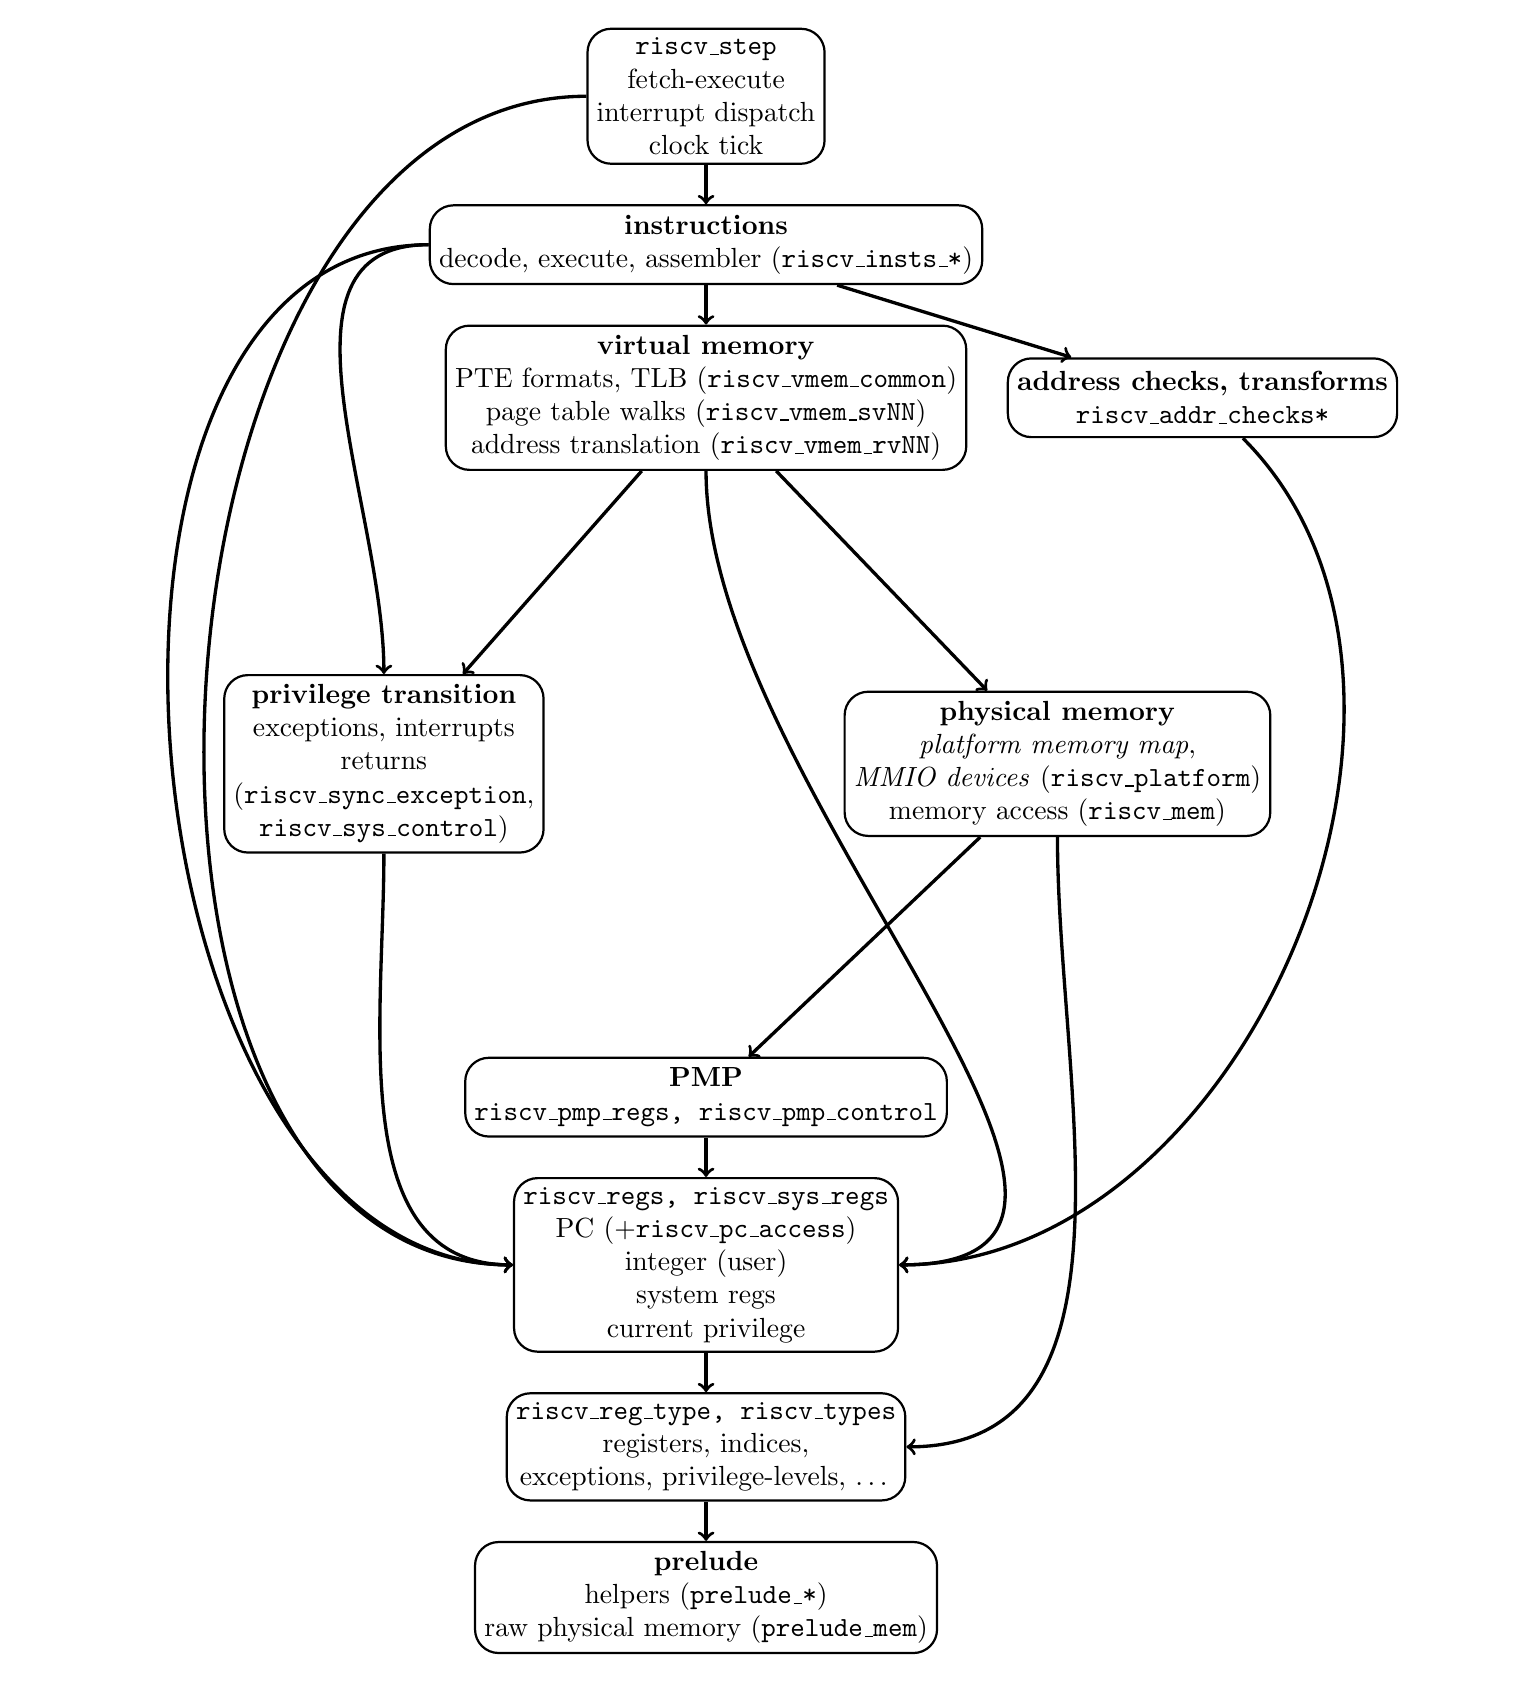
\begin{tikzpicture}[
    node distance=5mm,
    align=center,
    spec/.style={rectangle, rounded corners=3mm, minimum size=10mm,
      thick, draw=black},
    dep/.style={black, very thick}
  ]

  % layout the axial nodes

  \node (prelude) [spec]                         {\textbf{prelude}\\
                                                    helpers (\texttt{prelude\_*})\\
                                                    raw physical memory (\texttt{prelude\_mem})};
  \node (types)   [spec, above=of prelude]       {\texttt{riscv\_reg\_type, riscv\_types}\\
                                                    registers, indices,\\
                                                    exceptions, privilege-levels, \ldots};

  \node (regfile) [spec, above=of types]         {\texttt{riscv\_regs, riscv\_sys\_regs}\\
                                                    PC (+\texttt{riscv\_pc\_access})\\
                                                    integer (user)\\
                                                    system regs\\
                                                    current privilege};

  \node (pmp)     [spec, above=of regfile]       {\textbf{PMP}\\
                                                    \texttt{riscv\_pmp\_regs, riscv\_pmp\_control}};

  % compute location for virtmem
  \coordinate (vmloc) at ($(types)!3!(pmp)$);
  \node (virtmem) [spec] at (vmloc)              {\textbf{virtual memory}\\
                                                     PTE formats, TLB (\texttt{riscv\_vmem\_common})\\
                                                     page table walks (\texttt{riscv\_vmem\_svNN})\\
                                                     address translation (\texttt{riscv\_vmem\_rvNN})};


  % compute other relative locations for vertical alignment
  \coordinate (midpt) at ($(pmp.north)!0.5!(virtmem.south)$);
  \coordinate (exloc) at ($(midpt)!1.1!90:(virtmem.south)$);
  \coordinate (pmloc) at ($(midpt)!1.2!-90:(virtmem.south)$);

  \node (excepts) [spec] at (exloc)              {\textbf{privilege transition}\\
                                                    exceptions, interrupts\\
                                                    returns\\
                                                    (\texttt{riscv\_sync\_exception},\\
                                                    \texttt{riscv\_sys\_control})};

  \node (physmem) [spec] at (pmloc)              {\textbf{physical memory}\\
                                                     \textit{platform memory map},\\
                                                     \textit{MMIO devices} (\texttt{riscv\_platform})\\
                                                     memory access (\texttt{riscv\_mem})};



  \node (addrchk) [spec, right=of virtmem]       {\textbf{address checks, transforms}\\
                                                     \texttt{riscv\_addr\_checks*}};
  \node (insts)   [spec, above=of virtmem]       {\textbf{instructions}\\
                                                     decode, execute, assembler (\texttt{riscv\_insts\_*})};
  \node (fetch)   [spec, above=of insts]         {\texttt{riscv\_step}\\
                                                     fetch-execute\\
                                                     interrupt dispatch\\
                                                     clock tick};

  \draw[<-,dep] (prelude) edge (types);

  \draw[<-,dep] (types)   edge [out=0, in=270]    (physmem)
                          edge (regfile);

  \draw[<-,dep] (regfile) edge                    (pmp)
                          edge [out=180, in=270]  (excepts)
                          edge [out=0,   in=270]  (virtmem)
                          edge [out=180, in=180]  (insts)
                          edge [out=180, in=180]  (fetch);

  \draw[<-,dep] (pmp)     edge (physmem);

  \draw[<-,dep] (excepts) edge                  (virtmem)
                          edge [out=90, in=180] (insts);

  \draw[<-,dep] (addrchk) edge                   (insts)
                          edge [->,out=-45,in=0] (regfile);


  \draw[<-,dep] (physmem) edge (virtmem);

  \draw[<-,dep] (virtmem) edge (insts);

  \draw[<-,dep] (insts)   edge (fetch);

\end{tikzpicture}
\end{document}
